\documentclass[11pt,a4paper]{article}

\usepackage[utf8x]{inputenc}   % omogoča uporabo slovenskih črk kodiranih v formatu UTF-8
\usepackage[slovene]{babel}    % naloži, med drugim, slovenske delilne vzorce

\usepackage[hyphens]{url}
\usepackage{hyperref}

\usepackage{graphicx}



\title{Uporaba in analiza Monte-Carlo drevesnega preiskovanja na strateški igri\\
\textsc{dispozicija}}
\author{Jernej Habjan\\
jh0228@student.uni-lj.si\\
\ \\
predvideni MENTOR: doc. dr. Matej Guid \\
Fakulteta za računalništvo in informatiko Univerze v Ljubljani
\date{\today}         
}



\begin{document}
\maketitle

\begin{abstract}
Računalnik, ki igra proti človeškem nasprotniku lahko sprogramiramo na klasičen način pogoj - akcija. Tako so narejene klasične realno-časovno strateške igre, vendar gre veliko časa za implementacijo posameznih sovražnikovih napadov in nabiranju virov.
Lahko pa razvijemo algoritem, ki sam ugotovi, katera je optimalna odločitev v določeni situaciji in jo za tem izvede.
Na preprostih problemih z malo odločitvami in kratkimi igrami kot je igra križci in krožci, lahko izberemo preprostejše algoritme kot je algoritem Minimax, kjer igralec hoče povečati svojo možnost zmage, nasprotnik pa mu hoče to možnost zmanjšati.
Obstajajo tudi algoritmi, ki se naučijo igre iz učne množice, ki predstavlja nekaj iger, pri tem pa računalnik ugotovi zakonitosti igre in način igranja.
Taki algoritmi so nevronske mreže ali globoke nevronske mreže, ki pa so zelo računsko potratni, vendar vračajo izjemne rezultate. 
Lahko pa uporabimo algoritem Monte-Carlo drevesno preiskovanje, ki deluje na principu hevrističnega preiskovanja prostora, kjer imamo prostor stanj (graf, drevo), množico dosegljivih stanj in povezave med stanji.
Algoritem bom uporabil na svoji igri narejeni v celostnem pogonu Unreal Engine 4 imenovani Trump Defense 2020.
\end{abstract}


\section{Motivacija za izbrano diplomsko temo}

Razvijanje inteligentnega agenta v realno-časovnih igrah je problem, s katerim se mora soočiti večina razvijalcev teh iger, agentove akcije so pa pogosto predvidljive, saj se človeški igralec nauči njihovih načinov delovanja in jih tako lažje premaga.
Če pustimo agentu, da sam opravlja akcije nekontrolirano, bo izvajal naključne akcije, ki so pa slabše kot vnaprej definirana taktika.
Če pa agentu podamo hevristiko, po kateri se mora ravnati, bo poskušal izvesti čim boljše akcije, vendar bo to trajalo zelo dolgo, saj bo moral preiskati cel preiskovalni prostor, ki pa pri realno-časovnih strateških igrah zna biti zelo velik.
Da bi agent lahko poiskal cel prostor, bi ga morali zelo abstraktirati, vendar še takrat se moramo posluževati algoritmov kot je Monte-Carlo drevesno preiskovanje, ki uporablja naključnost, s katero se pomika skozi preiskovalni prostor.
S takim algoritmom lahko dosežemo inteligentnega agenta, ki se prilagaja nasprotnikovim akcijam, vsako igro izbira nov način igranja in deluje dovolj hitro brez daljšega učenja na superračunalnikih, kot to potrebujejo nevronske mreže.
Namen diplomske naloge je razviti algoritem na svoji realno-časovni strateški igri narejeni v celostnem pogonu Unreal Engine 4, ki bo dovolj inteligenten da premaga človeškega nasprotnika.

%Kaj je izhodišče za predlagano diplomsko temo? 
%Ali rešuje kakšen konkreten problem? 
%Ali demonstrira uporabo neke določene metode ali tehnologije?
%Ali izboljšuje dosedanji način dela na nekem področju?
%Komu bodo rezultati koristili?

\subsection{Pregled področja in sorodnih del}


Najbolj popularne tematike na področju igranja iger je sedaj računalniški program AlphaGo, ki uporabja kombinacijo globokih nevronskih mrež, strojnega učenja in drevesnega preiskovanja, in sicer Monte-Carlo drevesno preiskovanje.
Algoritem se je učil s pomočjo spodbujevalnega učenja, prav tako so pa algoritem naučili na podlagi 30 milijonov potez.
V oktobru 2017 so izdali novejšo verzijo AlphaGo Zero, ki pa ne uporablja znanja ekspertov, vendar se je algoritem naučil potez tako, da je igral sam proti sebi in tako premagal svojega predhodnika 100:0.\\

V delu Monte-Carlo tree search and rapid action value estimation in computer Go je opisana metodologija pri reševanju igre GO in metoda RAVE (Rapid action value estimation), ki spremlja število zmag v vseh dosedaj raziskanih vozliščih in to število vpliva na izbiro novega vozlišča~\cite{gelly2011monte}.


Uriarte z Drexel univerze je za uporabo Monte-Carlo drevesnega preiskovanja v dveh delih opisal abstrakcijo prostora in akcij.\\
V prvem delu je predstavil stanje, opisal okolico in abstrahiral mapo na posamezne dele, kjer ima vsak definirano svojo velikost~\cite{uriarte2014game}.
Leto pozneje je v delu Game-Tree Search over High-Level Game States in RTS Games predstavitev stanj in prosotra še izboljšal. Opredelil je še posamezne akcije, ki se zgodijo ob porazu vojske ali ob koncu igre~\cite{uriarte2015automatic}.





%Kaj je ``state of the art'' na področju diplomske naloge?
%Izberi nekaj najbolj sorodnih del in jih na kratko opiši!


\subsection{Zakaj je predlagani mentor primeren}

Izbral sem prof. doc. Mateja Guida, saj ima izkušnje z velikim kombinatoričnim prostorom, ki ga ponujata šah in realno-časovne strateške igre. Prav tako je pri šahu uporablal tehniko MCTS, ki jo bom jaz uporabil pri igri.
Realno-časovne strateške igre so predvsem strateške igre kot šah, vendar da se izvede toliko več ukazov, saj lahko namesto ene figure, premaknemo več figur v vsaki potezi. Tako da se bo problem, ki nastane pri igranju šaha lahko samo razširil na več figur na potezo.
Prav tako je predlagani mentor raziskal veliko različnih preiskovalnih algoritmov in mi bo lahko dal napotke, kako razširiti projekt z dodatnim algoritmom oziroma ga pripraviti na delujoče stanje z lažjim.



%Po kakšnih kriterijih si ga izbral?


%\clearpage
\section{Miselni diagram za izbrano temo diplomske naloge}

\begin{figure}[htb!]
\centerline{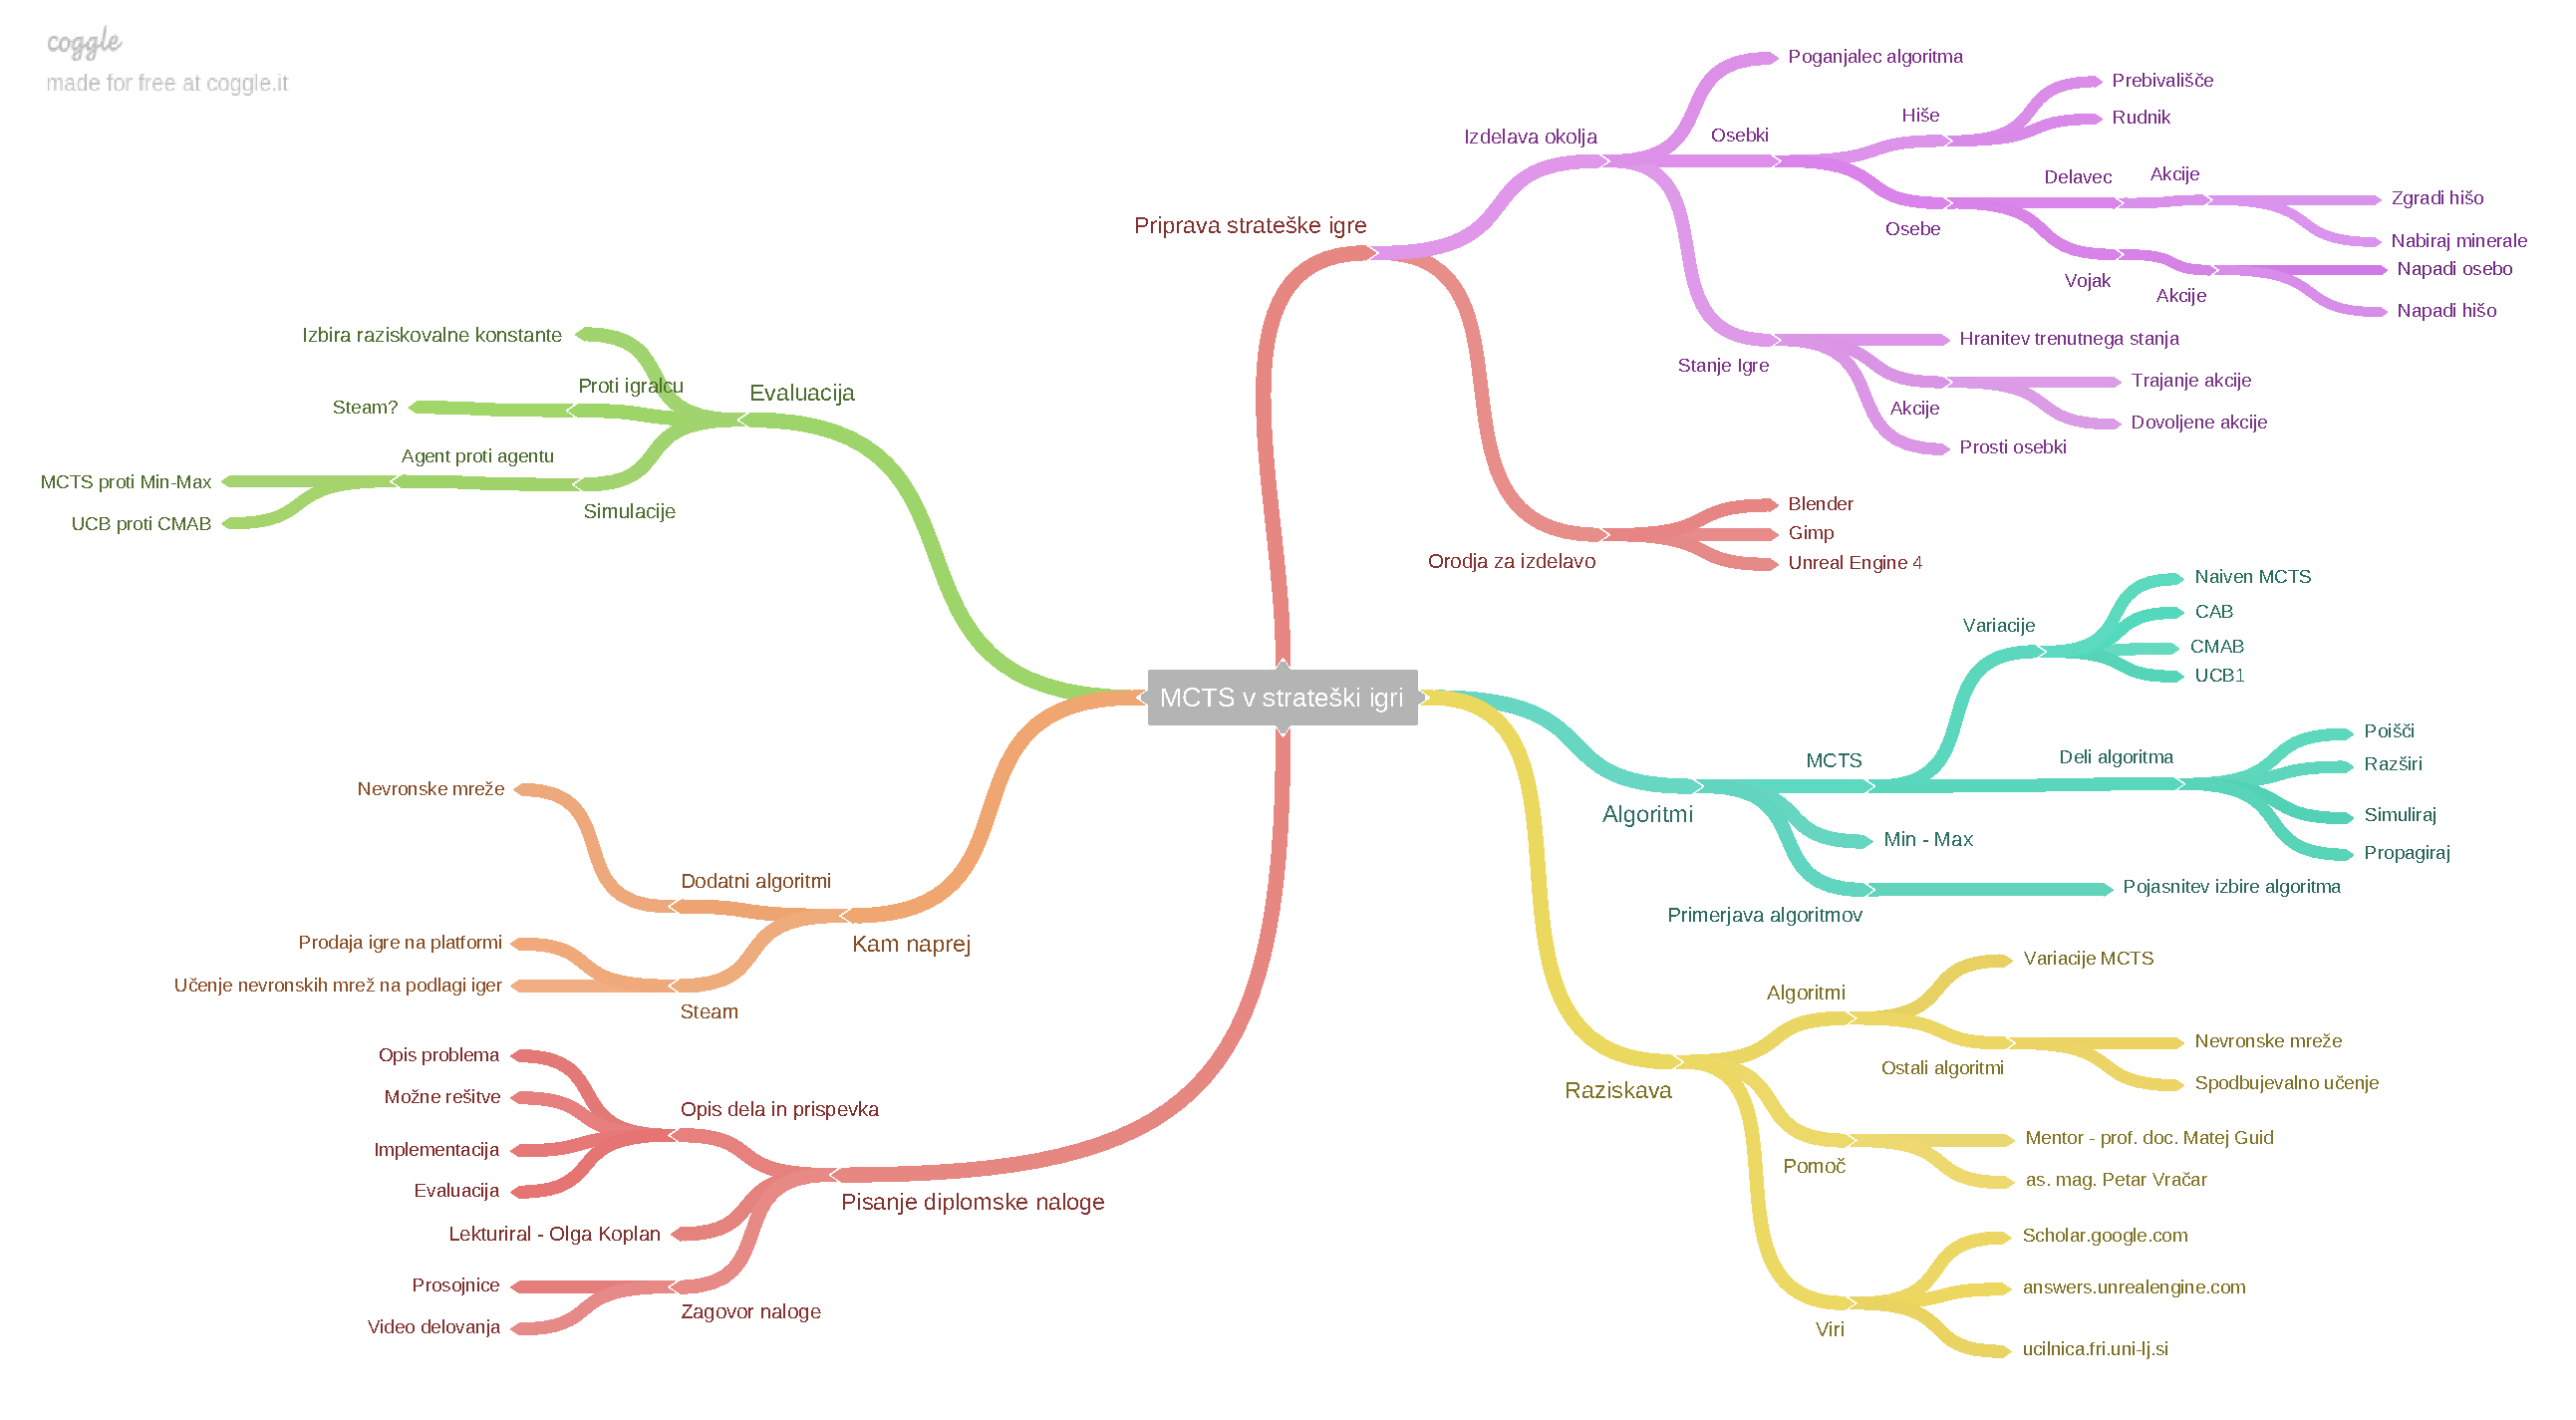
\includegraphics[height=0.5\textwidth, angle=0]{MCTS_v_strateki_igri.pdf}}
\caption{Miselni vzorec za mojo diplomsko nalogo.}
\label{sl:mindmap}
\end{figure}

Dopolnjen miselni vzorec (Slika \ref{sl:mindmap}).

%\clearpage

\section{Predvideni prispevki diplomske naloge}

Rezultat diplomske naloge bo realno-časovna strateška igra, ki ne vsebuje tradicionalega sprogramiranega inteligentnega agenta, vendar agenta, ki igra na podlagi nasprotnikovih akcij.
Rešitve, kot je naprimer število simulacij algoritma MCTS bom primerjal s številom simulacij v drugih igrah kot naprimer šah ali igri Micro-Rts in s tem preverjal hitrost delovanja algoritma.
Prav tako bom ocenil igranje računalnika proti računalniku z različnimi algoritmi in vodil statistiko igranja računalnika proti človeškim igralcem.



%Kaj bo rezultat diplomskega naloge? 
%Neka nova programska oprema, ki bo reševala določeno nalogo?
%Demonstracija neke obstoječe rešitve in metode na novem problemskem področju? 
%Kako boš uporabljene ali razvite rešitve v diplomi preveril?


\section{Uporabljena metodologija}


Za izdelavo igre bom uporabil celostno okolje Unreal Engine 4, v katerega bom uvažal 3D modele, narejene v programu Blender, ki pa potrebujejo za izgled teksturne slike, predelane v programu Gimp.
Algoritem bom razvijal prav tako v okolju Unreal Engine 4, ki pa ima podporo za kodiranje v programu Microsoft Visual Studio. V tem programu bom lahko pisal C++ kodo, ki je veliko hitrejša kot način programiranja v okolju Unreal Engine 4.
Preizkusiti nameravam hevristične algoritme, ki bodo izboljšali agentovo razmišljanje, kot naprimer Monte-Carlo drevesno preiskovanje in njegove variacije, spodbujevalno učenje in druge.
Testne podatke bom pa pridobil s člankov, v katerih je avtor uporabil te algoritme pri realno-časovnih strateških igrah. Tak podatek je število simulacij, ki pomeni hitrost algoritma in abstrakcija okolja.


%Katera orodja in razvojno okolje boš uporabil in zakaj? 
%Katere metode nameravaš preizkusiti?
%Kako boš pridobil testne podatke?


\section{Razdelitev potrebnega dela na aktivnosti}


\section{Potrebne aktivnosti za izdelavo moje diplomske naloge}
\begin{enumerate}
	\item \textbf{izdelava strateške igre}\\
	Igro moram izdelati v celostnem pogonu Unreal Engine 4.
	Igra bo realno-časovna, kar pomeni, da jo moram dobro optimizirati, če hočem poganjati hevristične preiskovalne algoritme. V tem okolju bom lažje zasnoval grafično prezentacijo algoritma.
	\begin{enumerate}
		\item izdelava poganjalca algoritma,
		\item izdelava osebkov,
		\item predelava stanja igre.
	\end{enumerate}
	Izdelati moram poganjalca algoritma, ki bo izbral določen algoritem in z njim igral proti nasprotniku.
	Prav tako moram izdelati osebke in njihove akcije (npr. postavi hišo).
	Te osebke bom pa hranil v stanju igre, ki pa ga algoritem uporablja, ki je abstrakcija za to, kateri osebki in akcije so trenutno na voljo.
	
	
	\item \textbf{raziskava algoritma}\\
	Ko bom imel izdelano ogrodje strateške igre, se bom lahko posvetil algoritmom.
	Preiskal bom algoritme:
	\begin{enumerate}
		\item Monte-Carlo drevesno preiskovanje,
		\item variacija Monte-Carla, in sicer Naiven MCTS,
		\item metode ocenjevanja CAB, UCB1,
	\end{enumerate}
	Prav tako bom moral hkrati opisati, zakaj sem se za kateri algoritem odločil.
	
	\item \textbf{implementacija algoritmov}\\
	Ko bom imel algoritem dokončan, ga bom lahko implementiral v igro.
	Postopek implementacije bo naslednji:
	\begin{enumerate}
		\item implementacija Min-Max algoritma,
		\item implementacija naključnega MCTS,
		\item sprememba MCTS, da uporablja pravilne ocene,
		\item sprememba preiskovalnega parametra pri ocenjevanju.
	\end{enumerate}
	
	\item \textbf{ovrednotenje rezultatov}\\
	Ovrednotenje rezultatov bo pa potekalo po naslednjih korakih:
	\begin{enumerate}
		\item simulacija igre računalnika proti računalniku (več sto simulacij),
		\item igranje računalnika proti človeku (testiranje znancev).
	\end{enumerate}
	Pri simulaciji računalnika proti računalniku, se bom osredotočil na rezultate kot so naprimer povprečno število simulacij pri MCTS algoritmu in konsistentnost ukazov.
	Pri igranju proti človeku bom pa analiziral nekaj odločitvenih dreves ki jih je računalnik zgeneriral in ocenil odločitve na podlagi mojega predznanja igre.
	
	\item \textbf{pisanje diplomske naloge}\\
	Pisanje diplomske naloge bo potekalo med raziskovanjem algoritmov in ovrednotenjem rezultatom.
	Prav tako bom opisal zakaj sem izbral določen algoritem in kaj mi doprinese k rezultatu.
	Opisal bom tudi celostni pogon Unreal Engine 4 in kratek opis strateške igre Trump Defense 2020.
	\item \textbf{zagovor}\\
	Za zagovor moram pripraviti prosojnice v Microsoft Office, ki bodo glavna podlaga pri prezentaciji.
	Prav tako bom moral pripraviti video, v katerem bom lahko predstavil igro in končen rezultat.
	
	
\end{enumerate}
Čas izdelave strateške igre bo med študijem trajal še kakšen mesec, je pa igra v izdelavi že dva meseca. Raziskava algoritmov bo hitrejša operacija, saj je potencialni mentor doc. Matej Guid v preteklosti že veliko delal s takimi algoritmi, in me bo hitro znal usmeriti.
Ta proces zna trajati kakšen teden, saj bom sproti dopolnjeval diplomsko nalogo.
Ko bom našel primerne algoritme, jih bom moral implementirati, kar pomeni, da bom moral predelati igro in hkrati testirati če algoritem dela. To lahko traja 2 meseca med študijem.
Potem bom moral še ovrednotiti rezultate, kar lahko traja tudi kakšen mesec, ker bom ugotovil, da algoritem ne dela dovolj dobro in ga bom spreminjal.
Diplomsko nalogo bom pa pisal en mesec.

Skupen čas celotnega projekta potem znaša približno 6 mesecev prekinjajočega dela.
Imam še štiri mesece dela za diplomsko nalogo, kar je spremenljiv čas, glede na to, da je še prvi semester.

Kritična aktivnost je implementacija algoritma, saj moram še dobro raziskati kako bi se lotil rešitve in vpeljati različne vrste algoritmov v realno-strateško igro. \\


%Sestavi spisek aktivnosti in podaktivnosti, ki te bodo pripeljale do konca diplome. Uporabi okolje ``enumerate''.
%Za vsako aktivnosti določi, katere aktivnosti morajo biti dokončane pred obravnavano aktivnostjo in  konkretno akcijo, ki bo začela reševati oziroma bo pokrenila aktivnost.

%Oceni trajanja vsake aktivnosti in posledično trajanje celotne izdelave diplomskega dela. Katere so kritične aktivnosti?


\section{Preliminarno kazalo}
\begin{enumerate}
	\item izdelava strateške igre
	\begin{enumerate}
		\item izdelava poganjalca algoritma,
		\item izdelava osebkov,
		\item predelava stanja igre.
	\end{enumerate}
	\item raziskava algoritma,
	\begin{enumerate}
		\item Monte-Carlo drevesno preiskovanje,
		\item variacija Monte-Carla, in sicer Naiven MCTS,
		\item metode ocenjevanja CAB, UCB1,
	\end{enumerate}
	\item implementacija algoritmov,
	\begin{enumerate}
		\item implementacija Min-Max algoritma,
		\item implementacija naključnega MCTS,
		\item sprememba MCTS, da uporablja pravilne ocene,
		\item sprememba preiskovalnega parametra pri ocenjevanju.
	\end{enumerate}
	\item ovrednotenje rezultatov,
	\begin{enumerate}
		\item simulacija igre računalnika proti računalniku (več sto simulacij),
		\item igranje računalnika proti človeku (testiranje znancev).
	\end{enumerate}
\end{enumerate}



%Sestavi preliminarno kazalo diplomske naloge. Razdelitev na poglavja in podpoglavja naredi v okolju ``enumerate'' in pri vsakem v enem ali dveh stavkih zapiši o čem bo poglavje govorilo.

%Celotna dispozicija naj bo dolga pet strani, vključno s slikami in seznamom literature.


\section{Seznam literature}

%Za izdelavo seznama literature uporabi  Bib\TeX!


\bibliographystyle{plain}
\bibliography{literatura}

\end{document}  




